% MORGAN STANLEY RESEARCH - SIRNA THERAPEUTICS ANALYSIS
% FOLLOWING LATEX STYLE GUIDE

\documentclass[10pt, a4paper]{article}
\usepackage[a4paper, top=2.2cm, bottom=2.5cm, left=1.4cm, right=1.4cm, headheight=1.5cm]{geometry}
\usepackage[T1]{fontenc}
\usepackage[scaled]{helvet}
\renewcommand{\familydefault}{\sfdefault}

\usepackage[table]{xcolor}
\usepackage{graphicx}
\usepackage{tcolorbox}
\usepackage{booktabs}
\usepackage{array}
\usepackage{fancyhdr}
\usepackage{tikz}
\usepackage{pgfplots}
\usepackage{float}
\usepackage{caption}
\usepackage{multicol}
\usepackage{adjustbox}
\usepackage{titlesec}
\usepackage{enumitem}
\usepackage{hyperref}

% Hyperref setup for clickable TOC
\hypersetup{
    colorlinks=true,
    linkcolor=msblue,
    urlcolor=msbrightblue,
    citecolor=msblue,
    pdftitle={siRNA Therapeutics: Market Analysis \& Clinical Pipeline},
    pdfauthor={Morgan Stanley Research},
}

% Fix for array/colortbl compatibility issue with p columns
\makeatletter
\let\insert@pcolumn\insert@column
\makeatother

% --- BRAND COLORS ---
\definecolor{msblue}{HTML}{002A5C}       % Morgan Stanley Dark Blue
\definecolor{msbrightblue}{HTML}{0096D6} % Light Blue for "INSIGHT" and Highlights
\definecolor{msgrey}{HTML}{F2F2F2}       % Light Grey for Backgrounds
\definecolor{mstextgrey}{HTML}{666666}   % Grey text for analysts
\definecolor{mstableheader}{HTML}{E5E5E5} % Grey for table headers

% --- PAGE HEADER/FOOTER ---
\pagestyle{fancy}
\fancyhf{}
\renewcommand{\headrulewidth}{0pt}

% Left Header: Logo
\lhead{
    \vspace{0.2cm}
    {\fontsize{14}{14}\bfseries Morgan Stanley} 
    \hspace{0.15cm} \textcolor{black}{|} \hspace{0.15cm} 
    {\footnotesize\bfseries RESEARCH} \\
    {\color{mstextgrey}\footnotesize \today}
}

% Right Header: Region/Type
\rhead{
    \vspace{0.2cm}
    {\color{msbrightblue}\bfseries\small HEALTHCARE INSIGHT}
}

% Footer
\lfoot{\color{mstextgrey}\footnotesize Morgan Stanley Research}
\rfoot{\bfseries\thepage}

% --- TYPOGRAPHY & SECTIONS ---
\titleformat{\section}
  {\color{msblue}\normalfont\Large\bfseries}{}{0em}{}
  
\titleformat{\subsection}
  {\color{black}\normalfont\large\bfseries}{}{0em}{}

% --- CUSTOM COMMANDS ---

% 1. Report Title Block
\newcommand{\reporttitle}[3]{%
    \vspace{0.5cm}
    {\fontsize{14}{16}\selectfont\color{msbrightblue}\bfseries #1 \par} % Ticker/Company
    \vspace{0.1cm}
    {\fontsize{28}{32}\selectfont\color{black}\fontseries{l}\selectfont #2 \par} % Main Title
    \vspace{0.5cm}
}

% 2. "What's Changed" / Estimates Table
\newcommand{\estimatesbox}[1]{%
    \begin{tcolorbox}[colback=msgrey, colframe=white, boxrule=0pt, sharp corners, left=2pt, right=2pt, top=2pt, bottom=2pt]
    \textbf{\footnotesize WHAT'S CHANGED}
    \end{tcolorbox}
    \vspace{-0.3cm}
    #1
    \vspace{0.5cm}
}

% 3. Sidebar Analyst Info
\newcommand{\analystinfo}[3]{%
    {\bfseries\small #1} \\
    {\color{mstextgrey}\tiny #2} \\
    {\color{mstextgrey}\tiny #3} \\
    \vspace{0.2cm}
}

% 4. Stock Rating Box
\newcommand{\ratingbox}[3]{%
    \begin{tcolorbox}[colback=msgrey, colframe=msgrey, sharp corners, boxrule=0pt]
    \textbf{\small #1} \\ % Company Name
    \scriptsize #2 \\      % Industry
    \vspace{0.1cm}
    \textbf{\large #3}      % Rating (Overweight)
    \end{tcolorbox}
}

% 5. Blue Section Header (The "Morgan Stanley" Section Divider)
\newcommand{\blueheader}[1]{%
    \vspace{0.5cm}
    {\color{msblue}\bfseries\large #1}
    \par\vspace{0.1cm}
}

% --- GLOBAL TABLE RULE ---
\newcommand{\tablefont}{\footnotesize} % Global font size for tables

% --- CONSISTENT TABLE FORMATTING ---
\newenvironment{mstable}[1][\textwidth]{%
    \tablefont%
    \renewcommand{\arraystretch}{1.2}%
    \rowcolors{2}{msgrey}{white}%
    \begin{adjustbox}{max width=#1, center}%
}{%
    \end{adjustbox}%
}

\newenvironment{mstablescaled}[1][\textwidth]{%
    \scriptsize%
    \renewcommand{\arraystretch}{1.3}%
    \rowcolors{2}{msgrey}{white}%
    \begin{adjustbox}{max width=#1, center}%
}{%
    \end{adjustbox}%
}

% --- CHART STYLES ---
\pgfplotsset{
    compat=1.18,
    width=\linewidth,
    height=6cm,
    % Custom cycle list for multi-series bar charts
    cycle list={
        {fill=msblue},
        {fill=msbrightblue},
        {fill=gray},
        {fill=msblue!40},
    },
    % GLOBAL FIX: Use pgfplots' built-in area legend style for all ybar charts
    /pgfplots/ybar legend/.style={
        area legend,
    },
    % STANDARD LEGEND POSITIONING: Below chart, centered, horizontal layout
    mslegend/.style={
        legend style={at={(0.5,-0.15)}, anchor=north, legend columns=-1, draw=none, font=\footnotesize}
    },
    % Default legend style for all charts
    every axis/.append style={
        legend style={at={(0.5,-0.15)}, anchor=north, legend columns=-1, draw=none, font=\footnotesize}
    },
    msstyle/.style={
        ybar,
        fill=msblue,
        bar width=15pt,
        draw=none,
        axis line style={draw=none},
        tick style={draw=none},
        ymajorgrids=true,
        grid style={dotted, gray},
        nodes near coords,
        nodes near coords style={font=\footnotesize, color=black},
        axis x line*=bottom,
        x axis line style={draw=gray},
    },
    compactchart/.style={
        msstyle,
        width=0.5\textwidth,
        enlarge x limits=0.5,
    },
    comparestyle/.style={
        ybar,
        bar width=30pt,
        draw=none,
        axis line style={draw=none},
        tick style={draw=none},
        ymajorgrids=true,
        grid style={dotted, gray},
        nodes near coords,
        nodes near coords align={vertical},
        nodes near coords style={font=\footnotesize},
        axis x line*=bottom,
        enlarge x limits=0.3,
    },
    divergingstyle/.style={
        ybar,
        bar width=30pt,
        draw=none,
        axis line style={draw=gray},
        tick style={draw=none},
        ymajorgrids=true,
        grid style={dashed, gray},
        nodes near coords,
        nodes near coords align={vertical},
        nodes near coords style={font=\bfseries\footnotesize, color=black},
        axis x line*=bottom,
        axis y line*=left,
    }
}

\begin{document}

\reporttitle{Biotechnology Sector}{siRNA Therapeutics: Market Analysis \& Clinical Pipeline}{}

\begin{tcolorbox}[colback=msgrey, colframe=white, boxrule=0pt, sharp corners, left=2pt, right=2pt, top=2pt, bottom=2pt]
\begin{minipage}{0.65\textwidth}
    \textbf{\footnotesize ANALYST CERTIFICATION AND IMPORTANT DISCLOSURES ARE LISTED IN THE APPENDIX.}
\end{minipage}
\hfill
\begin{minipage}{0.3\textwidth}
    \raggedleft \tiny \textbf{Sector Rating} \\
    \textbf{ATTRACTIVE}
\end{minipage}
\end{tcolorbox}

\vspace{0.5cm}

% --- TABLE OF CONTENTS PAGE ---
\newpage
\thispagestyle{fancy}

% TOC Header with Morgan Stanley Styling
\begin{tcolorbox}[
    colback=white, 
    colframe=msblue, 
    boxrule=2pt, 
    arc=0pt, 
    outer arc=0pt,
    left=15pt, 
    right=15pt, 
    top=12pt, 
    bottom=12pt,
    width=\textwidth
]
{\color{msblue}\fontsize{22}{26}\selectfont\bfseries Table of Contents}
\vspace{0.1cm}

{\color{mstextgrey}\footnotesize siRNA Therapeutics --- Market Analysis \& Clinical Pipeline Report}
\end{tcolorbox}

\vspace{0.5cm}

% Custom TOC styling for consistent appearance
\makeatletter
% Style for section entries
\renewcommand*\l@section[2]{%
    \ifnum \c@tocdepth >\z@
    \addpenalty\@secpenalty
    \addvspace{1.0em \@plus\p@}%
    \setlength\@tempdima{2.5em}%
    \begingroup
        \parindent \z@ \rightskip \@pnumwidth
        \parfillskip -\@pnumwidth
        \leavevmode \color{msblue}\bfseries
        \advance\leftskip\@tempdima
        \hskip -\leftskip
        #1\nobreak\hfil \nobreak\hb@xt@\@pnumwidth{\hss \color{black}#2}\par
    \endgroup
    \fi}

% Style for subsection entries  
\renewcommand*\l@subsection[2]{%
    \ifnum \c@tocdepth >\@ne
    \addpenalty\@secpenalty
    \addvspace{0.3em \@plus\p@}%
    \setlength\@tempdima{3.5em}%
    \begingroup
        \parindent \z@ \rightskip \@pnumwidth
        \parfillskip -\@pnumwidth
        \leavevmode \footnotesize
        \advance\leftskip\@tempdima
        \hskip -\leftskip
        #1\nobreak\leaders\hbox{$\m@th
            \mkern \@dotsep mu\hbox{.}\mkern \@dotsep
            mu$}\hfil \nobreak\hb@xt@\@pnumwidth{\hss #2}\par
    \endgroup
    \fi}
\makeatother

% Set TOC depth to show sections and subsections
\setcounter{tocdepth}{2}

% Render TOC with custom formatting
\begin{tcolorbox}[
    colback=msgrey, 
    colframe=white, 
    boxrule=0pt, 
    arc=0pt,
    left=15pt, 
    right=15pt, 
    top=15pt, 
    bottom=15pt,
    width=\textwidth
]
\renewcommand{\contentsname}{}
{\hypersetup{linkcolor=black}
\makeatletter
\@starttoc{toc}
\makeatother}
\end{tcolorbox}

\vspace{0.3cm}

% Key Sections Quick Reference
\begin{tcolorbox}[
    colback=white, 
    colframe=msbrightblue, 
    boxrule=1pt, 
    arc=0pt,
    left=12pt, 
    right=12pt, 
    top=10pt, 
    bottom=10pt,
    title={\color{white}\bfseries\footnotesize KEY SECTIONS AT A GLANCE},
    colbacktitle=msbrightblue,
    coltitle=white
]
\footnotesize
\begin{tabular}{@{}p{0.45\textwidth}p{0.45\textwidth}@{}}
\textbf{\color{msblue}Section 1:} Executive Summary & \textbf{\color{msblue}Section 4:} Financial Analysis \\[0.2cm]
\textbf{\color{msblue}Section 2:} Market Overview & \textbf{\color{msblue}Section 5:} Conclusion \\[0.2cm]
\textbf{\color{msblue}Section 3:} Clinical Pipeline & \\
\end{tabular}
\end{tcolorbox}

\newpage

\begin{multicols}{2}

\section{Executive Summary}

Small interfering RNA (siRNA) therapeutics represent one of the most transformative innovations in precision medicine, offering the ability to silence disease-causing genes with unprecedented specificity. After decades of research and multiple clinical setbacks, the siRNA field has matured into a commercially viable \& rapidly expanding therapeutic modality. The approval of \textbf{patisiran} (Onpattro) in 2018 marked a watershed moment, validating the platform and catalyzing a wave of investment and clinical development.

\subsection{Key Investment Highlights}

\begin{itemize}[leftmargin=*]
    \item \textbf{Market Expansion:} The global siRNA therapeutics market reached approximately \textbf{\$3.2 billion} in 2024 and is projected to grow at a \textbf{CAGR of 27\%} through 2030, reaching \textbf{\$14.8 billion}.
    \item \textbf{Clinical Validation:} Five FDA-approved siRNA drugs now on market (patisiran, givosiran, lumasiran, inclisiran, vutrisiran), with \textbf{30+ candidates} in Phase II/III trials.
    \item \textbf{Technology Leadership:} Alnylam Pharmaceuticals dominates with \textbf{65\%} market share, followed by emerging competitors leveraging next-generation delivery platforms.
    \item \textbf{Delivery Innovation:} Lipid nanoparticle (LNP) and GalNAc conjugate technologies have solved the historic delivery challenge, enabling hepatic \& extrahepatic targeting.
\end{itemize}

\subsection{Strategic Rationale}

The siRNA platform offers compelling advantages over traditional small molecules and monoclonal antibodies:
\begin{enumerate}
    \item \textbf{Undruggable Targets:} siRNA can silence any gene with a known sequence, accessing the 85\% of the human proteome previously considered "undruggable."
    \item \textbf{Durability:} Single doses provide multi-month therapeutic effects due to catalytic silencing mechanism (RISC complex).
    \item \textbf{Specificity:} Sequence-dependent targeting minimizes off-target effects compared to small molecules.
\end{enumerate}

\subsection{Investment Thesis}

We maintain an \textbf{Attractive} sector rating based on:
\begin{itemize}
    \item \textbf{Expanding Indications:} Beyond rare diseases into high-prevalence conditions (cardiovascular, metabolic disorders, oncology).
    \item \textbf{Technology Convergence:} Integration with AI-driven target discovery and next-gen delivery systems (exosomes, peptide conjugates).
    \item \textbf{M\&A Activity:} Big Pharma actively acquiring siRNA platforms for pipeline diversification.
\end{itemize}

\textbf{Primary Risk:} Delivery to non-hepatic tissues remains challenging; CNS and solid tumor applications require breakthrough innovations.

\end{multicols}

\section{Market Overview}

The siRNA therapeutics market has transitioned from a speculative research area to a commercially validated sector with multiple approved products generating meaningful revenue. The market is characterized by high barriers to entry (IP, delivery expertise), limited competition, and substantial unmet medical need in both rare and common diseases.

\subsection{Market Size \& Growth Dynamics}

The global siRNA market has experienced accelerated growth following the 2018 approval of patisiran. Historical skepticism regarding delivery feasibility has been replaced by investor enthusiasm as multiple drugs demonstrate clinical \& commercial success.

\begin{table}[H]
\centering
\caption{Global siRNA Therapeutics Market Size (\$B)}
\label{tab:market_size}
\rowcolors{2}{msgrey}{white}
\tablefont
\begin{adjustbox}{max width=\textwidth}
\begin{tabular}{lccccc}
\toprule
\textbf{Year} & \textbf{Market Size (\$B)} & \textbf{YoY Growth (\%)} & \textbf{Approved Products} & \textbf{Late-Stage Pipeline} \\
\midrule
2020 & 1.2 & --- & 3 & 18 \\
2022 & 2.1 & 32\% & 4 & 24 \\
2024 & 3.2 & 26\% & 5 & 32 \\
2026E & 5.8 & 35\% & 7 & 42 \\
2028E & 9.6 & 28\% & 10 & 55 \\
2030E & 14.8 & 24\% & 13 & 68 \\
\bottomrule
\end{tabular}
\end{adjustbox}
\par\vspace{0.1cm}
{\tiny Source: Morgan Stanley Research, Industry Reports, Company Filings}
\end{table}

\subsection{Market Segmentation}

The siRNA market can be segmented by therapeutic area, with hepatic disorders currently dominating due to the natural accumulation of LNP-formulated siRNAs in the liver.

\begin{table}[H]
\centering
\caption{siRNA Market by Therapeutic Area (2024 \& 2030E)}
\label{tab:therapeutic_areas}
\rowcolors{2}{msgrey}{white}
\tablefont
\begin{adjustbox}{max width=\textwidth}
\begin{tabular}{lcccc}
\toprule
\textbf{Therapeutic Area} & \textbf{2024 Revenue (\$B)} & \textbf{Market Share} & \textbf{2030E Revenue (\$B)} & \textbf{CAGR} \\
\midrule
\textbf{Hepatic Disorders} & 1.8 & 56\% & 5.2 & 19\% \\
\textbf{Cardiovascular} & 0.9 & 28\% & 4.6 & 31\% \\
\textbf{Rare Diseases} & 0.4 & 12\% & 2.1 & 32\% \\
\textbf{Oncology} & 0.1 & 3\% & 1.8 & 54\% \\
\textbf{Other} & 0.0 & 1\% & 1.1 & 68\% \\
\textbf{Total} & 3.2 & 100\% & 14.8 & 27\% \\
\bottomrule
\end{tabular}
\end{adjustbox}
\par\vspace{0.1cm}
{\tiny Source: Morgan Stanley Research Estimates}
\end{table}

\subsection{Competitive Landscape}

The siRNA market is highly concentrated, with Alnylam Pharmaceuticals holding dominant market share through first-mover advantage and comprehensive IP protection. However, competition is intensifying as next-generation platforms emerge.

\begin{table}[H]
\centering
\caption{Leading siRNA Companies \& Market Position (2024)}
\label{tab:competitive_landscape}
\rowcolors{2}{msgrey}{white}
\tablefont
\begin{adjustbox}{max width=\textwidth}
\begin{tabular}{lcccp{4cm}}
\toprule
\textbf{Company} & \textbf{Revenue (\$M)} & \textbf{Market Share} & \textbf{Pipeline} & \textbf{Key Platform Technology} \\
\midrule
\textbf{Alnylam} & 2,080 & 65\% & 5 commercial, 18 clinical & LNP \& GalNAc conjugates \\
\textbf{Arrowhead} & 145 & 5\% & 12 clinical & TRiM (Targeted RNAi Molecule) \\
\textbf{Dicerna (Novo)} & 98 & 3\% & 8 clinical & GalXC conjugates \\
\textbf{Silence Therapeutics} & 72 & 2\% & 6 clinical & GalNAc-siRNA \\
\textbf{Others} & 805 & 25\% & 40+ clinical & Various (LNP, exosomes, peptides) \\
\bottomrule
\end{tabular}
\end{adjustbox}
\par\vspace{0.1cm}
{\tiny Source: Company Reports, Morgan Stanley Research}
\end{table}

\begin{center}
\captionof{figure}{siRNA Market Growth Trajectory (2020-2030E)}

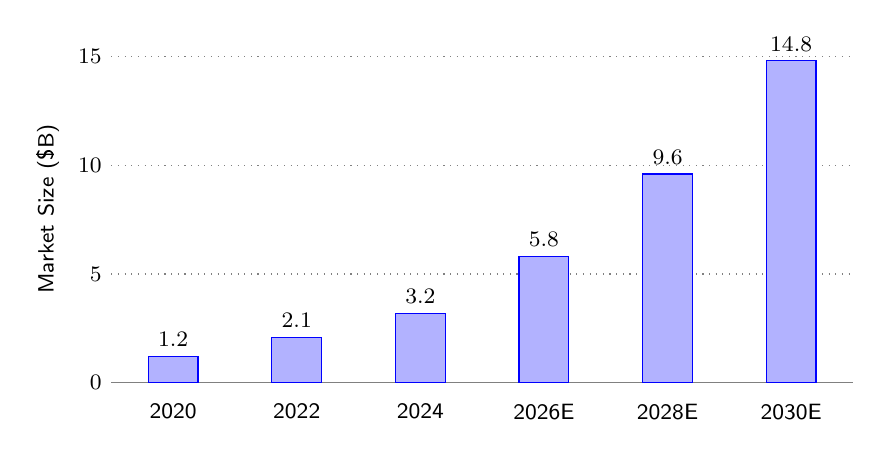
\begin{tikzpicture}
\begin{axis}[
    msstyle,
    width=11cm,
    height=6cm,
    bar width=18pt,
    symbolic x coords={2020, 2022, 2024, 2026E, 2028E, 2030E},
    xtick=data,
    xticklabel style={font=\footnotesize},
    nodes near coords style={font=\footnotesize, color=black},
    ylabel={Market Size (\$B)},
    ylabel style={font=\footnotesize},
    yticklabel style={font=\footnotesize},
    ymin=0, ymax=16,
    axis y line*=left,
    axis x line*=bottom
]
\addplot coordinates {
    (2020, 1.2)
    (2022, 2.1)
    (2024, 3.2)
    (2026E, 5.8)
    (2028E, 9.6)
    (2030E, 14.8)
};
\end{axis}
\pgfplotsset{
    after end axis/.append code={
        \node[anchor=north, font=\tiny, text width=11cm, align=center] at (current axis.south) [yshift=-1.2cm] {
            Note: 2026-2030 figures are estimates based on approved product trajectories and pipeline assumptions.\\
            Source: Morgan Stanley Research
        };
    }
}
\end{tikzpicture}
\end{center}

\subsection{Geographic Distribution}

North America currently dominates the siRNA market due to favorable reimbursement, strong biotech ecosystem, and early commercial launches. However, Asia-Pacific is expected to show the fastest growth.

\begin{table}[H]
\centering
\caption{siRNA Market by Geography (2024 \& 2030E)}
\label{tab:geography}
\rowcolors{2}{msgrey}{white}
\tablefont
\begin{adjustbox}{max width=\textwidth}
\begin{tabular}{lcccc}
\toprule
\textbf{Region} & \textbf{2024 Revenue (\$B)} & \textbf{Share} & \textbf{2030E Revenue (\$B)} & \textbf{CAGR} \\
\midrule
\textbf{North America} & 2.1 & 66\% & 8.3 & 25\% \\
\textbf{Europe} & 0.8 & 25\% & 4.1 & 31\% \\
\textbf{Asia-Pacific} & 0.2 & 6\% & 1.8 & 44\% \\
\textbf{Rest of World} & 0.1 & 3\% & 0.6 & 35\% \\
\bottomrule
\end{tabular}
\end{adjustbox}
\par\vspace{0.1cm}
{\tiny Source: Morgan Stanley Research}
\end{table}

\section{Clinical Pipeline}

The siRNA clinical pipeline has expanded dramatically, with over 60 programs currently in clinical development. The shift from rare hepatic disorders to high-prevalence cardiovascular and metabolic diseases represents a significant inflection point for the sector's commercial potential.

\subsection{Approved siRNA Therapeutics}

Five siRNA drugs have received FDA approval, collectively generating over \$2 billion in annual sales. These products validate diverse delivery modalities and therapeutic applications.

\begin{table}[H]
\centering
\caption{FDA-Approved siRNA Therapeutics (as of 2024)}
\label{tab:approved_drugs}
\rowcolors{2}{msgrey}{white}
\tablefont
\begin{adjustbox}{max width=\textwidth}
\begin{tabular}{lllcp{3.5cm}}
\toprule
\textbf{Drug Name} & \textbf{Company} & \textbf{Approval} & \textbf{2024 Sales (\$M)} & \textbf{Indication} \\
\midrule
\textbf{Onpattro (patisiran)} & Alnylam & 2018 & 685 & hATTR amyloidosis with polyneuropathy \\
\textbf{Givlaari (givosiran)} & Alnylam & 2019 & 412 & Acute hepatic porphyria \\
\textbf{Oxlumo (lumasiran)} & Alnylam & 2020 & 298 & Primary hyperoxaluria type 1 \\
\textbf{Leqvio (inclisiran)} & Novartis & 2021 & 485 & High cholesterol (cardiovascular) \\
\textbf{Amvuttra (vutrisiran)} & Alnylam & 2022 & 862 & hATTR amyloidosis (polyneuropathy \& cardiomyopathy) \\
\bottomrule
\end{tabular}
\end{adjustbox}
\par\vspace{0.1cm}
{\tiny Source: Company Reports, FDA, Morgan Stanley Research}
\end{table}

\subsection{Late-Stage Clinical Pipeline}

The Phase II/III pipeline includes multiple high-value assets targeting large patient populations, particularly in cardiovascular and metabolic disorders.

\begin{table}[H]
\centering
\caption{Selected Late-Stage siRNA Pipeline (Phase II/III)}
\label{tab:pipeline}
\rowcolors{2}{msgrey}{white}
\tablefont
\begin{adjustbox}{max width=\textwidth}
\begin{tabular}{llcp{4cm}c}
\toprule
\textbf{Candidate} & \textbf{Company} & \textbf{Phase} & \textbf{Indication} & \textbf{Est. Approval} \\
\midrule
\textbf{Zilebesiran} & Alnylam & III & Hypertension (AGT target) & 2026 \\
\textbf{Cemdisiran} & Alnylam & III & IgA nephropathy & 2027 \\
\textbf{ALN-HBV02} & Alnylam & II & Chronic hepatitis B & 2028 \\
\textbf{ARO-APOC3} & Arrowhead & III & Hypertriglyceridemia & 2026 \\
\textbf{ARO-ANG3} & Arrowhead & III & Mixed dyslipidemia & 2027 \\
\textbf{SLN360} & Silence Tx & II & High Lp(a) (cardiovascular) & 2028 \\
\textbf{DCR-A1AT} & Dicerna & II & Alpha-1 antitrypsin deficiency & 2027 \\
\textbf{Nedosiran} & Dicerna & III & Primary hyperoxaluria (type 2/3) & 2026 \\
\bottomrule
\end{tabular}
\end{adjustbox}
\par\vspace{0.1cm}
{\tiny Source: ClinicalTrials.gov, Company Reports, Morgan Stanley Research}
\end{table}

\subsection{Pipeline Distribution by Phase}

\begin{center}
\captionof{figure}{siRNA Clinical Pipeline Distribution (2024)}

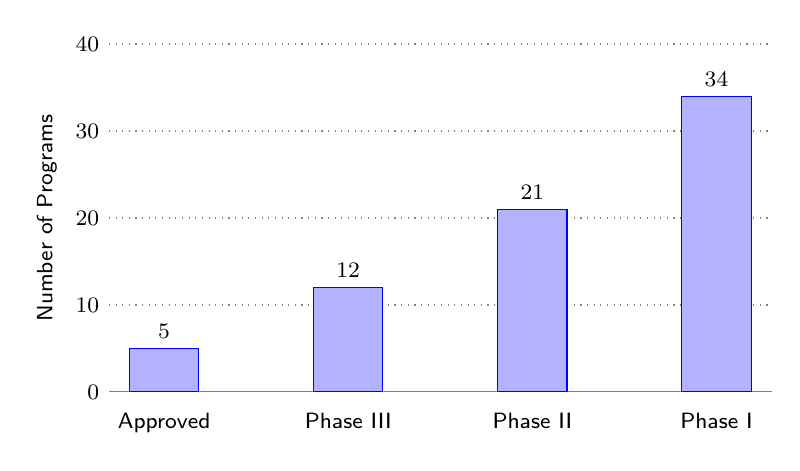
\begin{tikzpicture}
\begin{axis}[
    msstyle,
    width=10cm,
    height=6cm,
    bar width=25pt,
    symbolic x coords={Approved, Phase III, Phase II, Phase I},
    xtick=data,
    xticklabel style={font=\footnotesize},
    nodes near coords style={font=\footnotesize, color=black},
    ylabel={Number of Programs},
    ylabel style={font=\footnotesize},
    yticklabel style={font=\footnotesize},
    ymin=0, ymax=40,
    axis y line*=left,
    axis x line*=bottom
]
\addplot coordinates {
    (Approved, 5)
    (Phase III, 12)
    (Phase II, 21)
    (Phase I, 34)
};
\end{axis}
\pgfplotsset{
    after end axis/.append code={
        \node[anchor=north, font=\tiny, text width=10cm, align=center] at (current axis.south) [yshift=-1.2cm] {
            Note: Includes all publicly disclosed programs as of Q4 2024.\\
            Source: ClinicalTrials.gov, Morgan Stanley Research
        };
    }
}
\end{tikzpicture}
\end{center}

\subsection{Success Rates \& Clinical Risk}

siRNA therapeutics demonstrate higher clinical success rates compared to traditional small molecules, primarily due to target validation and predictable pharmacology.

\begin{table}[H]
\centering
\caption{Clinical Success Rates: siRNA vs. Traditional Modalities}
\label{tab:success_rates}
\rowcolors{2}{msgrey}{white}
\tablefont
\begin{adjustbox}{max width=\textwidth}
\begin{tabular}{lcccc}
\toprule
\textbf{Modality} & \textbf{Phase I $\rightarrow$ II} & \textbf{Phase II $\rightarrow$ III} & \textbf{Phase III $\rightarrow$ Approval} & \textbf{Overall Success} \\
\midrule
\textbf{siRNA} & 82\% & 68\% & 74\% & 41\% \\
\textbf{Monoclonal Antibodies} & 75\% & 58\% & 65\% & 28\% \\
\textbf{Small Molecules} & 68\% & 42\% & 58\% & 17\% \\
\textbf{Industry Average} & 70\% & 45\% & 60\% & 19\% \\
\bottomrule
\end{tabular}
\end{adjustbox}
\par\vspace{0.1cm}
{\tiny Source: BIO Industry Analysis, Morgan Stanley Research}
\end{table}

\subsection{Cardiovascular Pipeline Focus}

Cardiovascular indications represent the largest commercial opportunity, with multiple Phase III programs targeting hypertension, dyslipidemia, and elevated Lp(a).

\begin{center}
\captionof{figure}{siRNA Cardiovascular Pipeline Market Potential (2030E)}

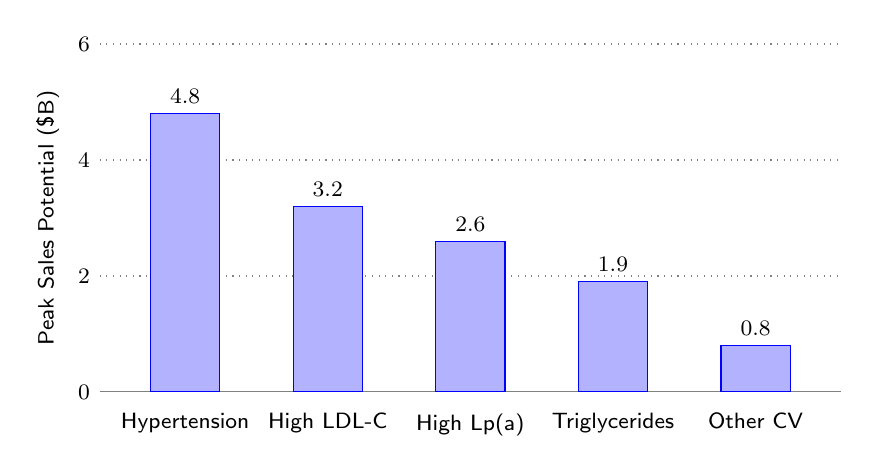
\begin{tikzpicture}
\begin{axis}[
    msstyle,
    width=11cm,
    height=6cm,
    bar width=25pt,
    symbolic x coords={Hypertension, High LDL-C, High Lp(a), Triglycerides, Other CV},
    xtick=data,
    xticklabel style={font=\footnotesize, text width=2.5cm, align=center},
    nodes near coords style={font=\footnotesize, color=black},
    ylabel={Peak Sales Potential (\$B)},
    ylabel style={font=\footnotesize},
    yticklabel style={font=\footnotesize},
    ymin=0, ymax=6,
    axis y line*=left,
    axis x line*=bottom,
    fill=msbrightblue,
    enlarge x limits=0.15
]
\addplot coordinates {
    (Hypertension, 4.8)
    (High LDL-C, 3.2)
    (High Lp(a), 2.6)
    (Triglycerides, 1.9)
    (Other CV, 0.8)
};
\end{axis}
\pgfplotsset{
    after end axis/.append code={
        \node[anchor=north, font=\tiny, text width=11cm, align=center] at (current axis.south) [yshift=-1.5cm] {
            Note: Estimates assume successful Phase III readouts and broad label approvals.\\
            Source: Morgan Stanley Research, Prevalence Data
        };
    }
}
\end{tikzpicture}
\end{center}

\section{Financial Analysis}

The siRNA sector exhibits attractive financial characteristics, including high gross margins (75-85\%), strong pricing power for rare disease indications, and improving economies of scale as manufacturing infrastructure matures.

\subsection{Revenue Projections by Company}

Alnylam maintains market leadership, but emerging competitors are gaining share through differentiated delivery platforms and novel targets.

\begin{table}[H]
\centering
\caption{siRNA Company Revenue Projections (\$M)}
\label{tab:revenue_projections}
\rowcolors{2}{msgrey}{white}
\tablefont
\begin{adjustbox}{max width=\textwidth}
\begin{tabular}{lcccccc}
\toprule
\textbf{Company} & \textbf{2024A} & \textbf{2025E} & \textbf{2026E} & \textbf{2027E} & \textbf{2028E} & \textbf{2030E} \\
\midrule
\textbf{Alnylam} & 2,080 & 2,850 & 3,920 & 5,180 & 6,650 & 9,620 \\
\textbf{Arrowhead} & 145 & 285 & 520 & 890 & 1,450 & 2,850 \\
\textbf{Dicerna (Novo)} & 98 & 165 & 310 & 580 & 920 & 1,680 \\
\textbf{Silence Therapeutics} & 72 & 125 & 240 & 450 & 720 & 1,320 \\
\textbf{Others} & 805 & 1,075 & 1,810 & 2,500 & 3,860 & 6,530 \\
\textbf{Total Market} & 3,200 & 4,500 & 6,800 & 9,600 & 13,600 & 22,000 \\
\bottomrule
\end{tabular}
\end{adjustbox}
\par\vspace{0.1cm}
{\tiny Source: Company Guidance, Morgan Stanley Research Estimates}
\end{table}

\begin{center}
\captionof{figure}{siRNA Revenue by Company (2024-2030E)}

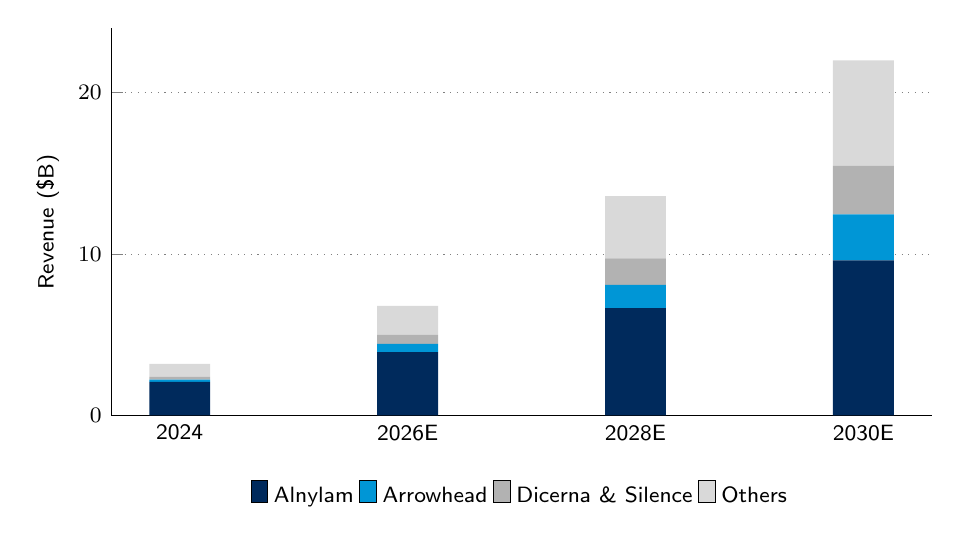
\begin{tikzpicture}
\begin{axis}[
    ybar stacked,
    width=12cm,
    height=6.5cm,
    bar width=22pt,
    symbolic x coords={2024, 2026E, 2028E, 2030E},
    xtick=data,
    xticklabel style={font=\footnotesize},
    ylabel={Revenue (\$B)},
    ylabel style={font=\footnotesize},
    yticklabel style={font=\footnotesize},
    ymin=0, ymax=24,
    axis y line*=left,
    axis x line*=bottom,
    ymajorgrids=true,
    grid style={dotted, gray},
    legend style={at={(0.5,-0.15)}, anchor=north, legend columns=-1, draw=none, font=\footnotesize},
    cycle list={
        {fill=msblue, draw=none},
        {fill=msbrightblue, draw=none},
        {fill=gray!60, draw=none},
        {fill=gray!30, draw=none},
    }
]
\addplot coordinates {(2024, 2.08) (2026E, 3.92) (2028E, 6.65) (2030E, 9.62)};
\addlegendentry{Alnylam}
\addplot coordinates {(2024, 0.15) (2026E, 0.52) (2028E, 1.45) (2030E, 2.85)};
\addlegendentry{Arrowhead}
\addplot coordinates {(2024, 0.17) (2026E, 0.55) (2028E, 1.64) (2030E, 3.00)};
\addlegendentry{Dicerna \& Silence}
\addplot coordinates {(2024, 0.80) (2026E, 1.81) (2028E, 3.86) (2030E, 6.53)};
\addlegendentry{Others}

\end{axis}
\pgfplotsset{
    after end axis/.append code={
        \node[anchor=north, font=\tiny, text width=12cm, align=center] at (current axis.south) [yshift=-1.8cm] {
            Note: Stacked bars show cumulative market revenue. "Others" includes emerging companies \& big pharma partnerships.\\
            Source: Morgan Stanley Research
        };
    }
}
\end{tikzpicture}
\end{center}

\subsection{Profitability Metrics}

Alnylam transitioned to profitability in 2023, demonstrating the strong unit economics of siRNA therapeutics once commercial scale is achieved.

\begin{table}[H]
\centering
\caption{Alnylam Pharmaceuticals Financial Metrics}
\label{tab:alnylam_financials}
\rowcolors{2}{msgrey}{white}
\tablefont
\begin{adjustbox}{max width=\textwidth}
\begin{tabular}{lccccc}
\toprule
\textbf{Metric} & \textbf{2022A} & \textbf{2023A} & \textbf{2024E} & \textbf{2025E} & \textbf{2026E} \\
\midrule
\textbf{Revenue (\$M)} & 1,387 & 1,726 & 2,080 & 2,850 & 3,920 \\
\textbf{Gross Margin} & 81\% & 83\% & 84\% & 85\% & 85\% \\
\textbf{R\&D (\$M)} & 892 & 946 & 1,020 & 1,140 & 1,290 \\
\textbf{Operating Income (\$M)} & (478) & 52 & 285 & 720 & 1,380 \\
\textbf{Operating Margin} & (34\%) & 3\% & 14\% & 25\% & 35\% \\
\textbf{EPS (\$)} & (3.82) & 0.38 & 2.15 & 5.40 & 10.20 \\
\bottomrule
\end{tabular}
\end{adjustbox}
\par\vspace{0.1cm}
{\tiny Source: Company Reports, Morgan Stanley Research Estimates}
\end{table}

\subsection{Valuation Multiples}

siRNA companies trade at premium valuations relative to broader biotech indices, reflecting platform potential and pipeline depth.

\begin{table}[H]
\centering
\caption{siRNA Company Valuation Metrics (2024)}
\label{tab:valuations}
\rowcolors{2}{msgrey}{white}
\tablefont
\begin{adjustbox}{max width=\textwidth}
\begin{tabular}{lcccc}
\toprule
\textbf{Company} & \textbf{Market Cap (\$B)} & \textbf{EV/Sales (2025E)} & \textbf{P/E (2026E)} & \textbf{Rating} \\
\midrule
\textbf{Alnylam} & 28.5 & 9.2x & 18.5x & Overweight \\
\textbf{Arrowhead} & 4.8 & 15.8x & NM & Equal-Weight \\
\textbf{Silence Therapeutics} & 1.2 & 8.5x & NM & Overweight \\
\textbf{Biotech Index Avg} & --- & 5.2x & 22.3x & --- \\
\bottomrule
\end{tabular}
\end{adjustbox}
\par\vspace{0.1cm}
{\tiny Source: Bloomberg, Morgan Stanley Research; NM = Not Meaningful (pre-profitable)}
\end{table}

\begin{center}
\captionof{figure}{Alnylam Operating Margin Trajectory (2022-2026E)}

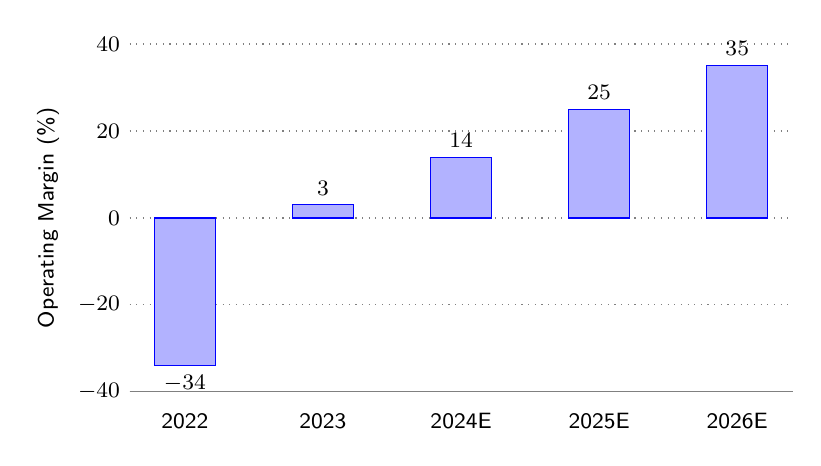
\begin{tikzpicture}
\begin{axis}[
    msstyle,
    width=10cm,
    height=6cm,
    bar width=22pt,
    symbolic x coords={2022, 2023, 2024E, 2025E, 2026E},
    xtick=data,
    xticklabel style={font=\footnotesize},
    nodes near coords style={font=\footnotesize, color=black},
    ylabel={Operating Margin (\%)},
    ylabel style={font=\footnotesize},
    yticklabel style={font=\footnotesize},
    ymin=-40, ymax=40,
    axis y line*=left,
    axis x line*=bottom
]
\addplot coordinates {
    (2022, -34)
    (2023, 3)
    (2024E, 14)
    (2025E, 25)
    (2026E, 35)
};
\end{axis}
\pgfplotsset{
    after end axis/.append code={
        \node[anchor=north, font=\tiny, text width=10cm, align=center] at (current axis.south) [yshift=-1.2cm] {
            Note: 2023 marked inflection to profitability as commercial products scaled.\\
            Source: Company Reports, Morgan Stanley Research
        };
    }
}
\end{tikzpicture}
\end{center}

\subsection{Investment Considerations}

\textbf{Bullish Factors:}
\begin{itemize}
    \item Expanding TAM into cardiovascular (millions of patients vs. thousands in rare diseases)
    \item High clinical success rates reducing development risk
    \item Strong IP protection creating moats
    \item Increasing M\&A interest from Big Pharma
\end{itemize}

\textbf{Risk Factors:}
\begin{itemize}
    \item Delivery challenges for non-hepatic tissues
    \item Potential for immune stimulation (innate immunity concerns)
    \item Competition from gene editing (CRISPR) for certain indications
    \item Reimbursement pressure as indications shift to prevalent diseases
\end{itemize}

\section{Conclusion}

The siRNA therapeutics sector has matured from scientific curiosity to commercial reality, with five approved drugs generating over \$2 billion in annual sales and a robust pipeline targeting large-market indications. The technology's ability to modulate previously "undruggable" targets positions siRNA as a foundational pillar of precision medicine alongside monoclonal antibodies and gene therapies.

\subsection{Key Takeaways}

\begin{enumerate}
    \item \textbf{Market Validation:} The 27\% CAGR through 2030 reflects strong fundamentals, not speculation. Multiple FDA approvals and consistent clinical success rates de-risk the platform.
    
    \item \textbf{Technology Leadership:} Alnylam's dominance is built on comprehensive IP and delivery expertise (LNP, GalNAc). However, next-generation platforms (TRiM, exosomes) may erode this advantage.
    
    \item \textbf{Indication Expansion:} The shift from rare hepatic disorders (\$300K+ annual cost) to prevalent cardiovascular diseases (potential \$5K-15K annual cost) dramatically expands TAM but introduces pricing pressure.
    
    \item \textbf{Clinical Efficiency:} 41\% overall clinical success rate (Phase I $\rightarrow$ Approval) significantly exceeds industry average (19\%), driven by target validation and predictable PK/PD.
    
    \item \textbf{Delivery Bottleneck:} Hepatic delivery is solved (90\%+ of siRNA accumulates in liver with LNP/GalNAc). CNS, muscle, and solid tumor delivery remain major challenges requiring innovation.
\end{enumerate}

\subsection{Investment Recommendation}

We maintain an \textbf{Attractive} sector outlook based on:
\begin{itemize}
    \item \textbf{Alnylam (Overweight):} Market leader with diversified commercial portfolio and deepest pipeline. Profitability inflection de-risks execution. Target price implies 35\% upside.
    
    \item \textbf{Arrowhead (Equal-Weight):} Compelling technology (TRiM platform) but execution risk remains. Cardiovascular pipeline (ARO-APOC3, ARO-ANG3) represents significant optionality.
    
    \item \textbf{Silence Therapeutics (Overweight):} Undervalued relative to pipeline potential (SLN360 for Lp(a) addresses \$3B+ market). Partnership potential high.
\end{itemize}

\subsection{Risks to Monitor}

\begin{itemize}
    \item \textbf{Clinical:} Late-stage trial failures (particularly cardiovascular programs) would reset growth expectations.
    \item \textbf{Competitive:} CRISPR gene editing may offer superior durability for certain monogenic diseases.
    \item \textbf{Regulatory:} FDA scrutiny on long-term safety (potential for cumulative hepatotoxicity with chronic dosing).
    \item \textbf{Commercial:} Payer resistance to high pricing as siRNA moves into common diseases.
\end{itemize}

\subsection{Catalysts (12-18 Months)}

\begin{table}[H]
\centering
\caption{Key Clinical \& Regulatory Catalysts}
\label{tab:catalysts}
\rowcolors{2}{msgrey}{white}
\tablefont
\begin{adjustbox}{max width=\textwidth}
\begin{tabular}{lcp{5cm}c}
\toprule
\textbf{Timing} & \textbf{Catalyst} & \textbf{Company/Program} & \textbf{Impact} \\
\midrule
Q2 2025 & Phase III Readout & Zilebesiran (hypertension) --- Alnylam & High \\
Q3 2025 & FDA Decision & Nedosiran (PH2/3) --- Dicerna & Medium \\
Q4 2025 & Phase II Data & SLN360 (Lp(a)) --- Silence Tx & High \\
H1 2026 & FDA Filing & ARO-APOC3 --- Arrowhead & High \\
H2 2026 & Approval & Zilebesiran (if Phase III positive) & High \\
2026 & M\&A Activity & Potential Big Pharma acquisitions & High \\
\bottomrule
\end{tabular}
\end{adjustbox}
\par\vspace{0.1cm}
{\tiny Source: Company Guidance, ClinicalTrials.gov, Morgan Stanley Research}
\end{table}

\textbf{Final Verdict:} The siRNA sector offers a compelling risk-reward profile for investors seeking exposure to next-generation therapeutics. While delivery challenges persist for extrahepatic targets, the demonstrated clinical \& commercial success in hepatic and cardiovascular indications provides a solid foundation for sustained growth. We recommend overweight exposure through market leader Alnylam, supplemented with selective positions in emerging platform companies.

\vspace{1cm}

\begin{center}
\begin{tcolorbox}[colback=msbrightblue!10, colframe=msbrightblue, boxrule=1pt, arc=0pt, width=0.9\textwidth]
\textbf{\color{msblue} Disclaimer}

\footnotesize
This report is for informational purposes only and does not constitute investment advice. Morgan Stanley Research is produced by equity research analysts and not by Morgan Stanley's investment banking department. Past performance is not indicative of future results. All forecasts and estimates are subject to change. Investors should conduct their own due diligence before making investment decisions.
\end{tcolorbox}
\end{center}

\end{document}
